\chapter{Marco teórico y Antecedentes }
\hrule \bigskip \vspace*{1cm}
%------------------------------------------------------------------------

\section{Desambiguación del sentido de las palabras (WSD)}
En general, la desambiguación del sentido de las palabras es el problema de seleccionar un sentido de un conjunto de posibilidades predefinidas para una palabra dada en un texto o discurso. 
En los últimos años se han incrementado las investigaciones para crear métodos de WSD. A continuación, se describe la clasificación para métodos de WSD de acuerdo a los recursos que utilizan (figura 2.1).

  \begin{figure}[h!]
	  \begin{center}
    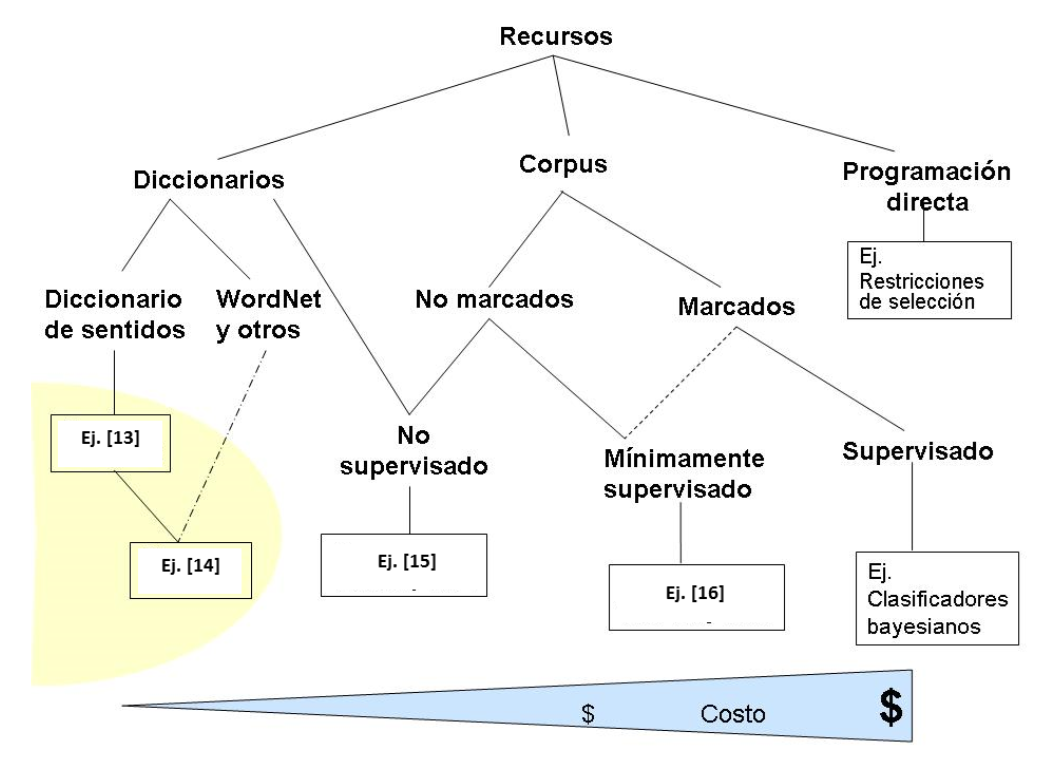
\includegraphics[angle=0, width=10cm]{Graficos/desambiguacion_WSD}
	  \caption{Clasificación de los métodos para WSD de acuerdo a los recursos que utilizan [1].}
    \end{center}
	\end{figure}

\section{Clasificación de sistemas en WSD}
\subsection{Métodos basados en conocimiento}
En esta categoría encontramos diferentes algoritmos para la etiquetación automática de sentidos. Normalmente, el rendimiento de estos métodos basados en conocimiento, es menor en comparación con los métodos basados en corpus. Pero con la salvedad de que los métodos basados en conocimiento tienen una amplia cobertura ya que pueden aplicarse a cualquier tipo de texto en comparación con los basados en corpus que sólo se pueden aplicar a aquellas palabras de las que se dispone de corpus anotados. A continuación, vamos a enumerar diferentes técnicas utilizadas por los métodos basados en conocimiento, aplicables sobre cualquier base de conocimiento léxica que defina sentidos de palabras y relaciones entre ellas. La base de conocimiento léxica más utilizada es WordNet (Miller (1995)). Vamos a describir 4 tipos diferentes de métodos basados en conocimiento:

\begin{itemize}
  \item Algoritmo de Lesk
  \item Similitud semántica
  \item Preferencias de selección
  \item Métodos Heurísticos
\end{itemize}

\subsubsection{Algoritmo de Lesk}
El algoritmo de Lesk [2] es uno de los primeros algoritmos exitosos usados en la desambiguación de sentidos de palabras. Este algoritmo se basa en dos puntos principales: un algoritmo de optimización para WSD y una medida de similitud para las definiciones de los sentidos.
El primer punto es acerca de desambiguar palabras considerando la coherencia global del texto, esto es, encontrar la combinación de los sentidos que maximice la relación total entre los sentidos de todas las palabras. 
Por ejemplo, para la oración \textit{My father deposits his money in a bank account} y considerando a lo más tres sentidos (véase tabla 1), para cada palabra, la figura 2 muestra la representación gráfica del algoritmo original de Lesk.

  \begin{figure}[h!]
    \begin{center}
    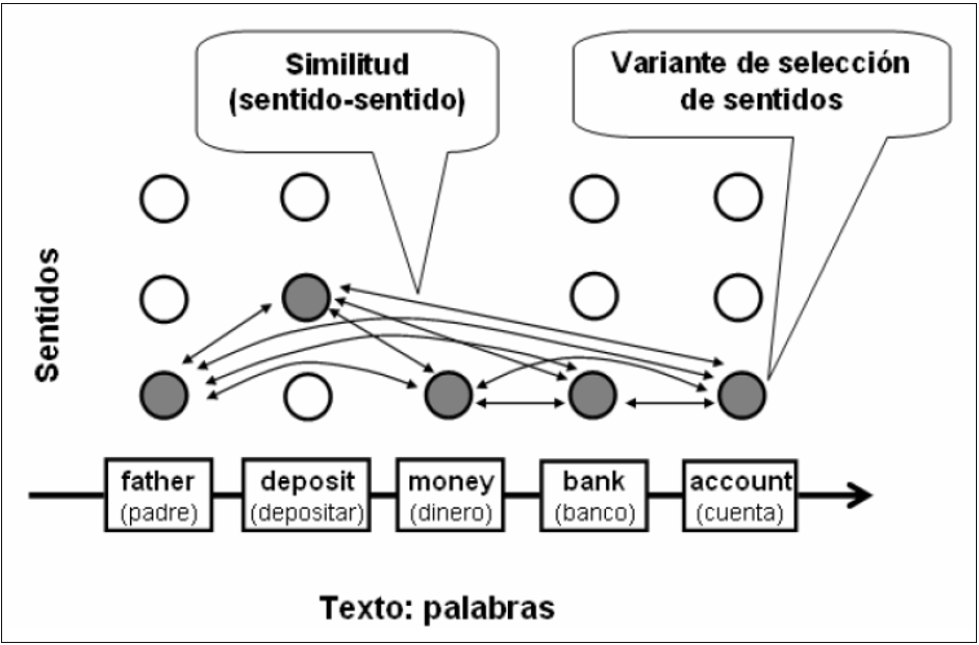
\includegraphics[angle=0, width=10cm]{Graficos/algoritmo_lesk}
    \caption{Representación gráfica del algoritmo original de Lesk [1]}
    \end{center}
  \end{figure}

  \begin{table}[t]
    \centering
      \begin{tabular}{|m{2cm}|m{10cm}|}
      \hline
      % after \\: \hline or \cline{col1-col2} \cline{col3-col4} ...
      Palabra & Sentidos\\
      \hline
      \hline
      Father & 1: a male parent (also used as a term of address to your father); "his father was born in Atlanta". 
      2: `Father' is a term of address for priests in some churches (especially the Roman Catholic Church or the Orthodox Catholic Church); “`Padre' is frequently used in the military”. 
      3: a person who holds an important or distinguished position in some organization; "the tennis fathers ruled in her favor"; "the city fathers endorsed the proposal".\\
      \hline
      Deposit & 1: fix, force, or implant; "lodge a bullet in the table". 
      2: put into a bank account; "She deposits her paycheck every month". 
      3: put (something somewhere) firmly; "She posited her hand on his shoulder"; "deposit the suitcase on the bench"; "fix your eyes on this spot".\\
      \hline
      Money & 1: the official currency issued by a government or national bank; "he changed his money into francs".  \\
      \hline
      Bank & 1: a financial institution that accepts deposits and channels the money into lending activities; "he cashed a check at the bank"; "that bank holds the mortgage on my home". 
      2: sloping land (especially the slope beside a body of water); "they pulled the canoe up on the bank"; "he sat on the bank of the river and watched the currents". 
      3: a supply or stock held in reserve for future use (especially in emergencies) \\
      \hline
      Account& 1: a formal contractual relationship established to provide for regular banking or brokerage or business services; "he asked to see the executive who handled his account". 
      2: the act of informing by verbal report; "he heard reports that they were causing trouble"; "by all accounts they were a happy couple". 
      3: a record or narrative description of past events; "a history of France"; "he gave an inaccurate account of the plot to kill the president"; "the story of exposure to lead".\\
      \hline
    \end{tabular}
    \caption{Sentidos de las palabras (máximo tres) obtenidas de WordNet para la oración \textit{“My father deposits his money in a bank account”}.[1]
    }\label{tab:demo}
  \end{table}

En el segundo punto, relacionado con la medida de similitud, Lesk sugiere usar el traslape entre las definiciones de los sentidos, es decir, contar el número de palabras que tienen en común. 
Como ejemplo, para la oración, \textit{“My father deposits his money in the bank ac-count”} para medir la relación de las definiciones de los sentidos para la palabra \textit{“de-posit”} y \textit{“bank”} como Lesk lo propuso, es necesario contar las palabras en común en todas las definiciones. En este caso, comparando principalmente las tres definiciones de \textit{“deposit”} contra las tres definiciones de “bank”. La relación entre los valores se muestra en la tabla 2.

\begin{table}[t]
  \centering
    \begin{tabular}{|m{4cm}|m{4cm}|m{4cm}|}
      \hline
      Sentido elegido para \textit{deposit} & Sentido elegido para \textit{bank} & Valor de relación (traslape de palabras)\\
      \hline
      1 & 1 & 0 \\
      \hline
      1 & 2 & 0 \\
      \hline
      1 & 3 & 0 \\
      \hline
      2 & 1 & 2 \\
      \hline
      2 & 2 & 1 \\
      \hline
      2 & 3 & 0 \\
      \hline
      3 & 1 & 1 \\
      \hline
      3 & 2 & 0 \\
      \hline
      3 & 3 & 0 \\
      \hline
     \end{tabular}
   \caption{Sentidos de las palabras (máximo tres) obtenidas de WordNet para la oración \textit{“My father deposits his money in a bank account”}.[1]
  }\label{tab:demo2}
\end{table}

Este algoritmo tiene dos limitaciones, por un lado, la limitación principal de la medida de similitud propuesta por Lesk, es que las glosas del diccionario, regularmente, son muy cortas y no incluyen el vocabulario suficiente para identificar los sentidos relacionados [3]. 
Por otro lado, mientras más palabras tenga el texto, y más sentidos por cada palabra, mayor será el número de combinaciones de sentidos, haciéndolo prácticamente prohibitivo para una búsqueda exhaustiva que garantice encontrar el óptimo global exacto. Por ejemplo, para una oración de 16 palabras de contenido, donde cada palabra contiene siete sentidos (números cercanos a los observados en el corpus de SemCor), existen 716 posibles combinaciones a escoger, de las cuales una será seleccionada. 
Debido a estas dos limitaciones, diferentes modificaciones al algoritmo original han sido propuestas para mejorar los resultados en la desambiguación de sentidos de palabras, las cuales se describen en la siguiente sección.

\begin{itemize}
  \item \textbf{Lesk simple o Lesk simplificado} \\
    Para reducir el espacio de búsqueda del algoritmo original de Lesk, Kilgarriff y Rosenzweig [4] propusieron una variación del algoritmo original de Lesk, conocido como algoritmo de \textbf{Lesk simplificado o Lesk simple}, donde los sentidos de las pala-bras en el texto son determinados uno a uno encontrando el mayor traslape entre los sentidos de las definiciones de cada palabra con el contexto actual, véase la figura 3. En lugar de buscar asignar, simultáneamente, el significado de todas las palabras en un texto dado, este enfoque determina el sentido de las palabras uno a uno, por lo que se evita la explosión combinatoria de sentidos.
  
    \begin{figure}[h!]
      \begin{center}
      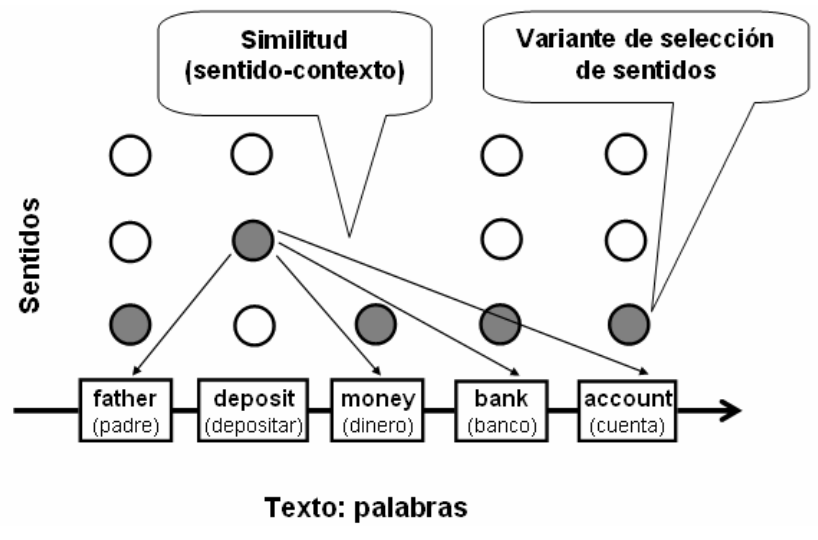
\includegraphics[angle=0, width=10cm]{Graficos/lesk_simple}
      \caption{Representación gráfica del algoritmo de Lesk simplificado [1]}
      \end{center}
    \end{figure}
    
    \item \textbf{Templado simulado (Simulated Annealing)} \\
    El método de templado simulado es una técnica para la resolución de problemas de optimización combinatoria a gran escala. El nombre de este algoritmo es una analogía del proceso metalúrgico en el cuál, el metal se enfría y se templa. La característica de este fenómeno es que en el enfriamiento lento alcanza una composición uniforme y un estado de energía mínimo, sin embargo, cuando el proceso de enfriamiento es rápido, el metal alcanza un estado amorfo y con un estado alto de energía. En templado simulado la variable \textbf{T} corresponde a la temperatura que decrece lentamente hasta encontrar el estado mínimo. 
    El proceso requiere una función \textbf{E}, la cual representa el estado de energía de cada configuración del sistema. Es esta función la que se intenta minimizar. A grandes rasgos el algoritmo funciona de la siguiente manera: se selecciona un punto inicial y además se escoge otra configuración de manera aleatoria, se calcula para ambas con-figuraciones su valor \textbf{E}, si el nuevo valor es menor que el seleccionado como punto inicial, entonces el inicial es remplazado por la nueva configuración. Una característica esencial del templado simulado es que, existe el caso en el que la nueva configuración es mayor a la configuración obtenida anteriormente, y la nueva es seleccionada. Esta decisión es tomada de manera probabilística y permite salir de algún mínimo local. Una vez que el método mantenga la misma configuración por un determinado tiempo, dicha configuración es escogida como la solución. 
    Cowie et al. [5], basándose en el algoritmo de Lesk, utilizó este método para desambiguación de sentidos de palabras de la siguiente forma: 
    \begin{enumerate}
      \item El algoritmo define una función \textbf{E} para la combinación de sentidos de palabras en un texto dado. 
      \item Se calcula \textbf{E} para la configuración inicial \textbf{C}, donde \textbf{C} es el sentido más frecuente para cada palabra.
      \item Para cada iteración, se escoge aleatoriamente otra configuración conocida como \textbf{C’}, y se calcula su valor de \textbf{E}. Si el valor de \textbf{E} para \textbf{C’} es menor que el de \textbf{C} entonces se elige \textbf{C’} como configuración inicial.
      \item  La rutina termina cuando la configuración de sentidos no ha cambiado en un tiempo determinado.
    \end{enumerate}
  
  \item Medida de Lesk Adaptada
    Lesk propuso medir la similitud entre sentidos contando el traslape de palabras. La limitación principal de esta técnica es que las glosas del diccionario, por lo general, son muy breves, de tal manera que no incluyen suficiente vocabulario para identificar los sentidos relacionados. En [6] se sugiere una adaptación del algoritmo basado en WordNet. Esta adaptación consiste en tomar en cuenta las glosas de los vecinos de la palabra a desambiguar, explotando los conceptos jerárquicos de WordNet, de tal ma-nera que las glosas de los vecinos son expandidas incluyendo a su vez las glosas de las palabras con las cuales se encuentran relacionadas mediante las diversas jerarquías que presenta WordNet. Así mismo, sugieren una variación en la manera de asignar el puntaje a una glosa, de tal manera que si “n” palabras consecutivas son iguales en ambas glosas, estas deberán de tener mayor puntaje que aquel caso en el que sólo coincide una sola palabra en ambas glosas. 
    Supongamos que \textit{bark} (ladrido o corteza) es la palabra que se desea desambiguar y sus vecinos son textit{dog} (perro) y textit{tail} (cola). El algoritmo original de Lesk verifica las coincidencias en las glosas de los sentidos de textit{dog} con las glosas de textit{bark}. Luego verifica las coincidencias en las glosas de textit{bark} y textit{tail}. El sentido de textit{bark} con el máximo número de coincidencias es seleccionado. La adaptación del algoritmo de Lesk consi-dera estas mismas coincidencias y añade además las glosas de los sentidos de los conceptos que se encuentran relacionados semántica o léxicamente a textit{dog}, textit{bark} y textit{tail}, de acuerdo a las jerarquías de WordNet.
\end{itemize}

\subsubsection{Similitud semántica}
\subsubsection{Preferencias de selección}
\subsubsection{Métodos Heurísticos}

\subsection{Métodos basados en corpus no supervisados}
El desarrollo de métodos que tratan de resolver el problema de la ambigüedad léxica ha supuesto la aparición de diferentes algoritmos que utilizan una serie de recursos diferentes. Podemos encontrar desde sistemas que utilizan técnicas de enriquecimiento de conocimiento utilizando diccionarios, tesauros o jerarquías de conceptos (los llamados basados en conocimiento), hasta sistemas que utilizan la información de textos anotados semánticamente (los llamados sistemas supervisados basados en corpus). El único inconveniente de estos sistemas es que es necesario la creación de textos, diccionarios u otras fuentes de información, de forma manual.
Esto supone un gran costo en su obtención y mantenimiento, además de generar dificultades cuando se tratan de anotar textos muy extensos, de un nuevo dominio o de un lenguaje diferente. Para evitar esta dependencia se han desarrollado dos aproximaciones diferentes. La primera de ellas trata de establecer distinciones entre sentidos basándose en su distribución, determinando por tanto que, palabras que aparecen en contextos similares deben tener sentidos similares [7]y [8]. La segunda aproximación está basada en equivalencias de traducción en corpus paralelos, los cuales identifican traducciones de una palabra en un lenguaje determinado cuya traducción depende del sentido de esa palabra en el lenguaje origen. Estas traducciones dependientes del sentido de una palabra pueden ser utilizadas como una recopilación de sentidos para esa palabra en el lenguaje origen.
Una de las claves de los métodos basados en distribución, es que no utilizan ningún recopilatorio de sentidos, únicamente clasifican palabras basándose en sus contextos observados en los corpus. Esta es una alternativa a los métodos que dependen de la anotación de corpus y que están restringidos a aquellas palabras que un experto ha clasificado para sus distintos sentidos. En todo caso, a pesar de que exista un repertorio de sentidos, su utilidad depende de las aplicaciones sobre las que se aplique. Las aproximaciones distribucionales no asignan sentidos a las palabras, pero sí permiten discriminar entre los sentidos de una palabra identificando clusters en contextos similares, donde cada cluster muestra que una palabra se está utilizando con un sentido determinado. Estos métodos presentan una aproximación diferente a la tarea tradicional de WSD, la cual clasifica palabras con respecto a un repertorio de sentidos existente. Los métodos basados en equivalencias de traducción se basan en el hecho de que los sentidos diferentes de una palabra en un lenguaje origen se pueden traducir en palabras diferentes en el lenguaje destino. Estas aproximaciones tienen dos propiedades. Primero, automáticamente derivan un repertorio de sentidos que hace distinciones relevantes para los problemas de traducción automática. Segundo, un corpus etiquetado basado en estas distinciones puede ser creado automáticamente y utilizado como corpus de entrenamiento para los métodos tradicionales de aprendizaje supervisado.
Una de las ventajas de utilizar métodos no supervisados basados en corpus, es que no se basan en ningún diccionario, repositorio de sentidos, tesauro, etc. De forma que no están restringidos a la interpretación de sentidos que el autor del diccionario haya impuesto. Ya que, es muy habitual que diferentes diccionarios aporten una distinción de sentidos más fina o más compacta, según la finalidad para la que estén creados. Al evitar hacer uso de estos recursos, se garantiza la adaptabilidad de estos sistemas a diferentes campos o ámbitos. Otra ventaja no menos importante, es que estos métodos son independientes del lenguaje. Es decir, son fácilmente adaptables a cualquier idioma que disponga de un corpus sobre el que obtener información.

\subsubsection{Métodos distribucionales}
Este tipo de métodos identifican las palabras que suelen aparecer en contextos similares, sin necesidad de utilizar un repositorio de sentidos. En [9] por ejemplo, se realiza el proceso de desambiguación en dos pasos. El primer paso, es construir clusters que comparten características similares. El segundo paso, es etiquetar cada cluster con una definición que establezca el sentido de la palabra dentro de ese contexto. Esta es una visión completamente diferente del concepto general de WSD, donde los sentidos se suponen conocidos antes de comenzar el proceso de desambiguación. Esta nueva visión de “discriminación y etiquetación” corresponde a la forma ideal de obtener la definición de una palabra (lexicografía). Un lexicógrafo, seleccionaría diferentes contextos de una palabra determinada, a partir de un corpus extenso y representativo para el usuario final. Por ejemplo, si hablamos de un diccionario para niños, el corpus consistiría en textos escritos para niños. Y si hablamos de un diccionario sobre un dominio específico el corpus deberían ser textos de esa especialidad en particular. De esta forma el lexicógrafo, dividiría los contextos en los que aparece la palabra a estudiar en diferentes clusters, discriminando los diferentes sentidos que puede adoptar esa palabra, sin tener ninguna idea preconcebida de cuántos sentidos puede adoptar. El resultado de la discriminación es un número determinado de clusters que establecen los diferentes sentidos de la palabra, obtenidos estos a partir del corpus de entrada. A partir de aquí, se debe estudiar cada cluster y obtener una definición que actúe como una etiqueta o un sentido específico para la palabra. Esta última parte, la de asignar una definición concreta a la palabra en cada cluster es la más problemática, dado que en muchas ocasiones es difícil establecer una definición a partir de los contextos. Una posible solución sería identificar el conjunto de palabras que aparecen en un cluster y utilizarlas como una aproximación al sentido de la palabra. Por ejemplo, si tenemos la palabra “línea” y un cluster con: “teléfono”, “llamada”, “ocupada”, “móvil”. En este caso, estas palabras son indicativas del sentido asociado a este cluster. De esta forma, si los métodos no supervisados basados en corpus son desarrollados eficientemente, el resultado podría llegar a ser un proceso independiente del lenguaje que resuelve el problema de la ambigüedad sin tener que recurrir a un repositorio de sentidos. Existen dos aproximaciones distintas para los métodos distribucionales: Discriminación basada en tipos. Estos métodos identifican conjuntos (o clusters) de palabras que pueden estar relacionadas entre sí debido a su aparición en contextos similares. Normalmente se basan en medidas de similitud entre vectores de co-ocurrencia. Discriminación basada en tokens. Estos métodos agrupan todos los contextos donde una palabra determinada aparece, basándose en la similitud de estos contextos.

\subsubsection*{Discriminación basada en tipos}
En el caso de los métodos de discriminación basados en tipos, es necesario disponer de corpus extensos para poder extraer la similitud entre diferentes contextos donde aparece la palabra a desambiguar. En estos métodos la representación más utilizada se basa normalmente en la contabilización de co-ocurrencias o en medidas de asociación entre palabras. Usando esta información es posible identificar otras palabras que aparecen en contextos similares y por tanto pueden tener sentidos similares. De esta forma, se pueden extraer los distintos sentidos que puede adoptar una palabra polisémica. Por ejemplo, si seleccionamos la palabra “línea” que puede tener varios sentidos (línea telefónica, trazo, premio en el juego del bingo, etc), y ésta aparece en dos contextos distintos: contexto1 (dibujo, trazo, color, coordenada) y contexto2 (auricular, teléfono, comunicar, llamada). Podemos establecer a partir de las palabras extraídas del contexto, que en el primer caso “línea” hace referencia a un trazo en un dibujo, y en el segundo caso, hace referencia a una línea telefónica. Como ya se ha mencionado anteriormente, los métodos distribucionales basados en tipos necesitan de corpus bastante extensos. Es por ello, que la representación del espacio contextual se realizará en matrices de NxN dimensiones, donde N, es el número de palabras en el corpus. Cada celda de esta matriz contiene el número de veces que las palabras representadas en cada columna y fila co-ocurren dentro de una ventana de un tamaño especificado. Cuando no importa el orden en el que aparecen las palabras la frecuencia será la misma, pero si hablamos de bigramas, donde el orden sí importa, el valor de las celdas será distinto. Por tanto, si el orden no importa, se tendrá   cuadrada y simétrica. Sin embargo, si tenemos en cuenta el orden de aparición de las palabras, tendremos una matriz rectangular y no simétrica. Para estas matrices de co-ocurrencia, las celdas pueden almacenar el número de veces que dos palabras co-ocurren, o también pueden tomar valores más complejos. Por ejemplo, las celdas de una matriz de co-ocurrencia pueden contener el valor de diferentes medidas de asociación como: log-likelihood ratio [10] o Información Mutua [11]. Estas medidas indican el grado en que dos palabras co-ocurren con respecto a las demás palabras del corpus. En el caso de la medida del log-likelihood ratio partimos de una tabla 2 x 2 como sigue a continuación Tabla 2.7.

\begin{table}
  \centering
  \begin{tabular}{|l|c|c|c|}
    \hline
     & Corpus 1 & Corpus 2 & Total \\
    \hline
    Frecuencia de la palabra & a & b & a + b \\
    \hline
    Frecuencia de otras palabras & c - a & d - b & c + d - a - b \\
    \hline
    Total & c & d & c + d \\
    \hline
  \end{tabular}
  \caption{Tabla 2x2 para log-likelihood ratio [12]}
  \label{tab:demo3}
\end{table}

En la Tabla 2.7 se extraen las frecuencias relativas de una palabra entre dos corpus. Se denota por c al número de palabras total del corpus1 y por d al número de palabras total del corpus2 (N en total). Los valores de a y b son denotados como valores observados (O). Por último, queda por definir los valores esperados (E), según la Fórmula 2.15.

\begin{equation}
E_i=\frac{N_i\displaystyle\sum_{i}^{} O_i}{\displaystyle\sum_{i}^{} N_i}
\end{equation}

Para la Tabla 2.7 $N_1 = c$ y $N_2 = d$. Por lo tanto, para la palabra que estamos tratando:

\begin{equation}
  E_1=\frac{c*(a+b)}{(c+d)}\hspace{1cm} \text{y}\hspace{1cm} E_2=\frac{d*(a+b)}{(c+d)}
\end{equation}

Los cálculos para obtener los valores esperados tienen en cuenta el tamaño de los dos corpus. Por tanto, no es necesario normalizar los valores, pudiendo aplicar a continuación la medida del log-likelihood según la Fórmula 2.3

\begin{equation}
  -2\ln\lambda=2\displaystyle\sum_{i}^{} O_i\ln \left(\frac{O_i}{E_i}\right)
\end{equation}

La Fórmula 2.3 es equivalente a calcular el log-likelihood ratio $G^2$ como sigue:

\begin{equation}
  G^2=2*\left(a*\ln \left(\frac{a}{E_1}\right)\right)+\left(b*\ln \frac{b}{E_2}\right)
\end{equation}

Si los valores esperados y los observados son comparables, el valor de $G^2$ estará próximo a 0, lo que significa que la palabra ha aparecido junto a otra por casualidad, y no están relacionadas entre sí. Si se obtiene un valor mayor que 0, significa que los valores observados difieren en gran medida de los valores esperados, por lo que las palabras estarán fuertemente relacionadas entre sí.
Una vez decidido el tipo de medida a utilizar para establecer la co-ocurrencia entre distintas palabras y construida la matriz de co-ocurrencia, cada palabra será representada como un vector de N-dimensiones. A partir de cada vector obtenido, se puede medir la similitud contextual entre dos palabras obteniendo el coseno entre los vectores. Para el cálculo del coseno entre dos vectores se utiliza la Fórmula 2.5

\begin{equation}
  \cos (\vec{x},\vec{y})=\frac{\vec{x}\cdot\vec{y}}{|\vec{x}|\times |\vec{y}|}
\end{equation}

Continuando con la definición de métodos distribucionales basados en tipos, encontramos distintos algoritmos que pueden ser aplicados. En esta sección vamos a tratar dos de estos algoritmos: Análisis de la Semántica Latente (LSA) [13] y Clustering by Committee (CBC) [14]. Mediante el algoritmo de LSA se representa un corpus en un espacio multidimensional, usando vectores. Cada vector representará el contexto en el cual aparece una palabra. En el caso de LSA no se hacen distinciones entre los distintos sentidos de una palabra polisémica, es decir, se formará un único vector para cada palabra, aunque ésta tenga varios sentidos diferentes. Usando la información del contexto, se podrá determinar, por ejemplo, que palabras como: coche, automóvil, auto... están relacionadas semánticamente.

Cuando hablamos de LSA, debemos pensar en la representación del conocimiento como matrices de [ palabras-contextos]. Para medir el grado de similitud de una palabra con respecto a otras palabras del contexto, se utiliza la medida del coseno entre vectores. Además de poder comparar palabras y contextos, también se puede medir el grado de similitud entre oración-oración, contexto-contexto... simplemente calculando el vector resultado de la unión de cada uno de los vectores que conforman las palabras de la oración, del contexto, etc. Mediante el algoritmo de CBC se pueden detectar clusters de palabras relacionadas con los distintos sentidos de una palabra polisémica. Por ejemplo, para la palabra “muñeca” el algoritmo de CBC podría identificar dos clusters, uno asociado con el sentido de juguete, con palabras como juego, entretenimiento, niños, cochecito, etc, y otro cluster asociado con el sentido de parte del cuerpo humano, con palabras como brazo, extremidad, articulación, etc. Por lo tanto, con el algoritmo de CBC se pueden detectar palabras sinónimas asociadas a los diferentes sentidos de una palabra. Ambos algoritmos, tanto LSA como CBC, utilizan representaciones multidimensionales de co-ocurrencia de palabras.

\subsubsection*{Discriminación basada en tokens}

El objetivo de este tipo de métodos es agrupar los contextos en los que una palabra aparece bajo el mismo sentido. A continuación, se van a describir métodos que utilizan características de primer y segundo orden. Las características de primer orden ocurren directamente en un contexto que está siendo clasificado, mientras que las características de segundo orden son aquellas que ocurren junto con una de primer orden, pero no ocurren en el contexto que está siendo clasificado. En primer lugar, es necesario establecer cómo se van a representar los contextos que van a ser clasificados en clusters. Al igual que para los sistemas supervisados, los contextos contienen la palabra a desambiguar con la excepción de que esta no tiene asignado ningún sentido. La premisa de los métodos basados en tokens es que si una palabra aparece en contextos similares ésta ha de tener el mismo sentido.
Uno de los primeros métodos que utilizó discriminación basada en tokens fue una adaptación del algoritmo de LSA usando características de segundo orden [9]. En este caso, la representación de la matriz de co-ocurrencia en lugar de utilizar palabras utiliza contextos completos usando co-ocurrencias de segundo orden de características léxicas. Una palabra tiene una co-ocurrencia de segundo orden con otra, cuando ambas no aparecen juntas, pero ambas sí aparecen junto a otra palabra frecuentemente. Por ejemplo, en “policía de tráfico” y “accidente de tráfico”, la palabra “policía” es una co-ocurrencia de segundo orden de “accidente”, porque ambas co-ocurren en primer orden con “tráfico”. Otro método que utiliza esta aproximación es el de [15]. En este caso, utilizan un conjunto reducido de características de primer orden para crear matrices que muestran la similitud entre contextos. Estas características se extraen a partir de las palabras que se encuentran alrededor de la palabra a desambiguar e incluyen etiquetas sintácticas y palabras co-ocurrentes.
El problema de este tipo de métodos es la forma de evaluación de los resultados. Debido a que la discriminación no parte de un conjunto preestablecido de sentidos, no se puede evaluar la forma en que los nuevos sentidos son descubiertos, sobretodo si se está trabajando en un dominio específico.

\subsection{Métodos basados en corpus supervisados}
\subsection{Métodos híbridos}
